\section{COT Trigonometric Cotangent Function}

\subsection{Usage}

Computes the \verb|cot| function for its argument.  The general
syntax for its use is
\begin{verbatim}
  y = cot(x)
\end{verbatim}
where \verb|x| is an \verb|n|-dimensional array of numerical type.
Integer types are promoted to the \verb|double| type prior to
calculation of the \verb|cot| function.  Output \verb|y| is of the
same size and type as the input \verb|x|, (unless \verb|x| is an
integer, in which case \verb|y| is a \verb|double| type).  
\subsection{Function Internals}

Mathematically, the \verb|cot| function is defined for all 
arguments \verb|x| as
\[
  \cot x \equiv \frac{\cos x}{\sin x}
\]
For complex valued arguments \verb|z|, the cotangent is computed via
\[
  \cot z \equiv \frac{\cos 2 \Re z + \cosh 2 \Im z}{\sin 2 \Re z + 
  i \sinh 2 \Im z}.
\]
\subsection{Example}

The following piece of code plots the real-valued \verb|cot(x)|
function over the interval \verb|[-1,1]|:
@>


\centerline{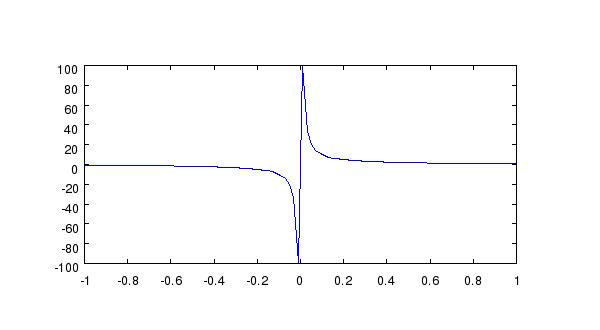
\includegraphics[width=8cm]{cotplot}}

